\documentclass[11pt, twocolumn]{article}
\usepackage{fullpage}
\usepackage{url}
\usepackage{graphicx}
\usepackage{pdftexcmds}
\usepackage{listings}
\begin{document}

\title{Processing USPTO Patent Data}
\author{Gabe Fierro\\
	Coleman Fung Institute for Engineering Leadership\\
	UC Berkeley\\
	\texttt{fierro@eecs.berkeley.edu}}
\date{\today}
\maketitle

\begin{abstract}
We describe a completely automated data process designed to consume weekly releases of patent grants and applications distributed by the United States Patent and Trademark Office (USPTO). The process downloads and unpacks the zipped distribution files, parses the raw data into a SQL database, and performs various disambiguations and statistical calculations on the database.
\end{abstract}

\section{Introduction}
Patent data plays an invaluable role in research into economic trends,
invention, innovation policy and technology strategy. Since the digitization of
patent data starting in 1975, though patent data has been freely available
through the United States Patent and Trademark Office, it has been difficult to
use. We present a substantial improvement in data quality and accessibility
over previous third-party re-releases of US patent data. This will not only
facilitate further research on up-to-date patent records, but also increase the
reproducibility of previous research results.

\section{Processing Workflow}
\begin{figure*}
\center 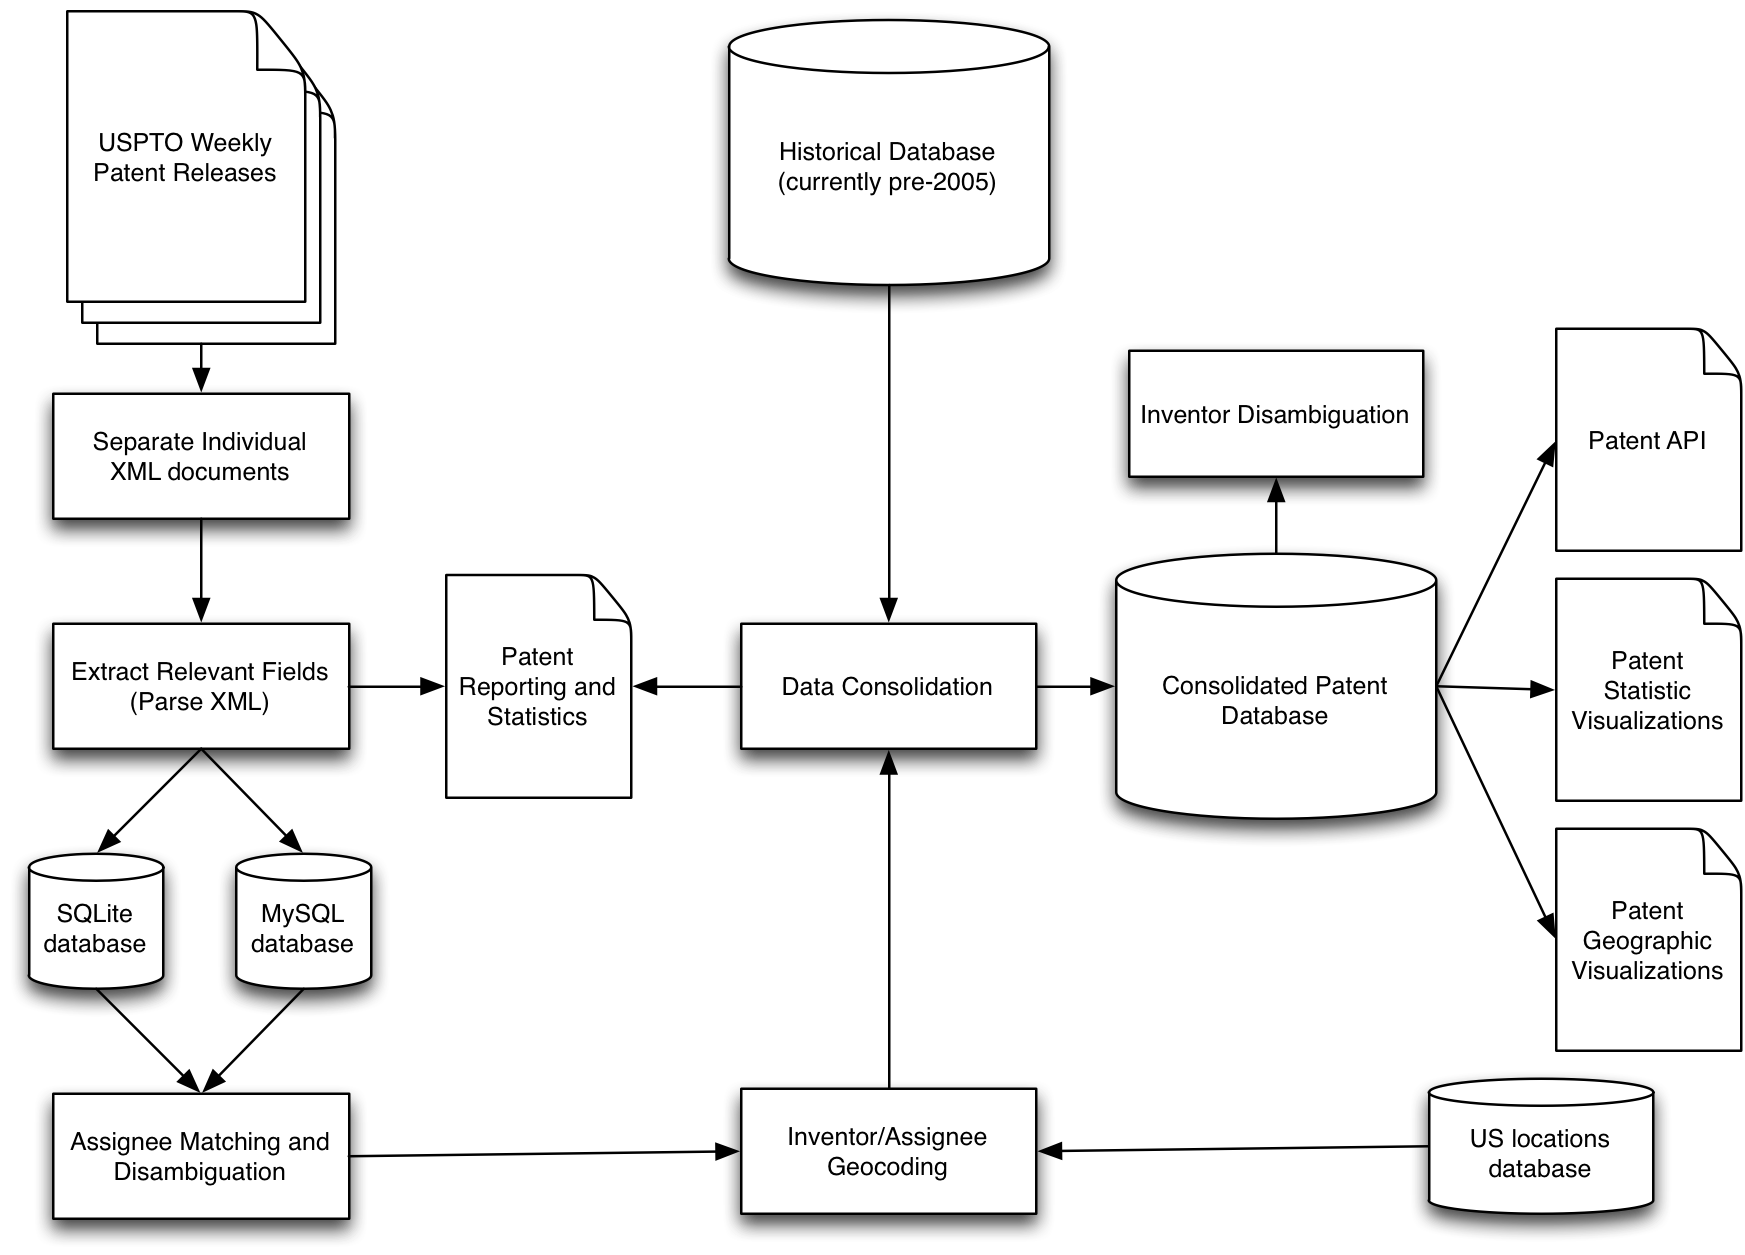
\includegraphics[width=0.8\textwidth]{figs/dataprocess}
\caption{Full patent data process flow}


\label{fig:dataprocess} 
\end{figure*}


The Fung Institute has developed a robust and fully automated toolchain
for processing and providing high quality patent data intended for
research, as illustrated in Figure~\ref{fig:dataprocess}.

As data is downloaded from the USPTO weekly patent releases, it is
parsed, cleaned and inserted into a SQL database. From this database,
assignee and lawyer disambiguations are performed and the patents
are geocoded with a location-based disambiguation. The output data
from these processes are combined with the historical data from the
Harvard Dataverse Network into a single consolidated database. From
this database, an inventor-level disambiguation can be performed,
and various applications can take advantage of the completed data.

\section{Data Sources}
The unified patent dataset is composed of processed data from two
separate sources: the Harvard Dataverse Network (DVN)~\cite{disambiguation}
collection of patent data from 1975 through 2010 and the weekly distributions
of Google-hosted USPTO records~\cite{googlefiles}\cite{googlefiles-applications}.


\subsection{Harvard DVN}

The Harvard DVN patent database consists of data drawn from the National
Bureau of Economic Research (NBER), weekly distributions of patent
data from the USPTO, and to a small extent, the 1998 Micropatent CD
product~\cite{micropatent}. The schema of the database can be found
in the Appendix.

While the Harvard DVN patent database was, prior to the UC Berkeley
patent database, the most extensively complete amalgamation of United
States patent data, it is not without its problems. Firstly, there
is little information as to the actual meanings of the columns in
the databases. Without sufficient prior knowledge of patent structure,
it is difficult to glean the semantic significance of each column.
The names alone are often abbreviated and hard to discern. Secondly,
because the DVN database is a combination of several sources into
a single database schema, certain patent entries from NBER and Micropatent
are incomplete where their data source did not provide all the requisite
data. The data obtained from the weekly distributions suffers from
being made available in several different formats. The parser that
was developed to handle the data is overly complicated and does not
handle edge cases well, resulting in missing patent metadata where
the parser did not account for a subtle change in format~\cite{oldparser}.
This is analyzed in greater detail below.


\subsection{USPTO Weekly Distributions}

\begin{table*}[t]
\center %
\begin{tabular}{|l|l|}
\hline 
Time Span  & Data Format \tabularnewline
\hline 
-1974  & paper-based \tabularnewline
1975  & unknown. Data obtained from Micropatent \tabularnewline
1976 - 2001  & Green Book (CITE) APS key-value \tabularnewline
2001  & SGML ST. 32 v2.4 \tabularnewline
2002 - 2004  & Red Book (CITE) XML ST. 32 v2.5 \tabularnewline
2005  & Red Book XML ST. 36 (ICE) v4.0 \tabularnewline
2006  & Red Book XML ST. 36 (ICE) v4.1 \tabularnewline
2007 - 2012  & Red Book XML ST. 36 (ICE) v4.2 \tabularnewline
2013  & Red Book XML ST. 36 (ICE) v4.3 \tabularnewline
2013 -  & Red Book XML v4.4 \tabularnewline
\hline 
\end{tabular}\caption{Table of USPTO grant data formats}


\label{fig:grantformats} 
\end{table*}
\begin{table*}[t]
\center %
\begin{tabular}{|l|l|}
\hline 
Time Span  & Data Format \tabularnewline
\hline 
-2001 & paper-based \tabularnewline
2001  & XML ST. 32 v1.5\tabularnewline
2002 - 2004  & Red Book (CITE) XML ST. 32 v1.6 \tabularnewline
2005 & Red Book XML ST. 36 (ICE) v4.0\tabularnewline
2006 & Red Book XML ST. 36 (ICE) v4.1 \tabularnewline
2007 - 2012 & Red Book XML ST. 36 (ICE) v4.2 \tabularnewline
2013 -  & Red Book XML ST. 36 (ICE) v4.3\tabularnewline
\hline 
\end{tabular}\caption{Table of USPTO grant data formats}


\label{fig:applicationformats} 
\end{table*}


The USPTO distributions take the form of zip archives containing concatenated
XML (Extensible Markup Language) documents, each of which contains
the full text of each patent grant and patent application issued every
week. Prior to 1975, the USPTO used a purely paper-based system before
transitioning to a raw-text key-value and later SGML-based key-value
store %
\footnote{Standard Generalized Markup Language%
}. Patent documents were made available in the XML format starting
in 2001. Although this data is made freely available, the fact that
digital USPTO patent data spans eight different formats and occupies
more than 70 GB (compressed) over the 37 years of its existence makes
rendering the data into an amenable form a nontrivial problem (see
Table~\ref{fig:grantformats} and Table~\ref{fig:applicationformats}).
Patent application data, though only available in a digital format
back to 2001, is nonetheless available in six different formats~\cite{xmlresources}~\cite{xmlretrospective}.

\section{Parsing}
The process of converting the public patent data into a usable form
begins with parsing, the manipulation of a document's grammar and
anatomy to extract structured and labeled data. The Fung Institute
parser takes as input the weekly USPTO patent distributions and outputs
the relevant data into a SQL database. To simplify the problem of
parsing the diversity of formats of digital patent data, the current
parser addresses only the XML-based documents. At time of writing,
the Fung Institute parser is capable of handling patent grants of
formats XML v4.0, v4.1, v4.2, v4.3 and v4.4 (spanning 2005 through
2013) and patent applications of formats XML v1.5, v1.6, v4.0, v4.2
and v4.3 (spanning 2001 through 2013). Grant data prior to 2005 is
drawn from a truncated version of the Harvard DVN database.

The code is written in Python 2~\cite{python} and is available on
Github~\cite{newparser}.

\begin{figure*}[t]
\center 

\begin{verbatim}
<applicants>
    <applicant sequence="001" app-type="applicant-inventor"> 
        <addressbook> 
            <last-name>Roach</last-name>
            <first-name>Richard</first-name>
            <address>
                <city>Schaumburg</city>
                <state>IL</state>
                <country>US</country>
            </address>
        </addressbook>
    </applicant>
    <applicant sequence="002" app-type="applicant-inventor"> 
        ...
    </applicant>
</applicants>
\end{verbatim}

\caption{Sample inventor element from XML v4.2 schema}


\label{fig:inventorelement} 
\end{figure*}



\subsection{XML Overview}

XML, or Extensible Markup Language, defines a set of rules for encoding
documents that seek to facilitate comprehension by both machines and
humans. Since the publishing XML 1.0 standard in 1996, the format
gained traction due to the minimal size and flexible structure. In
its simplest form, an XML document is a collection of elements, which
are each composed of tags and content. Tags, such as \verb`<citation>`,
lend semantic structure to a document and allow a reader to determine
the significance of the content that follows. An element is a logical
component that begins and ends with tags (e.g. \verb`<citation>`
and \verb`</citation>`) and contains either regular text or additional,
nested elements. An example of an element can be found in Figure~\ref{fig:inventorelement}.


\subsection{Parser Method}

The Fung Institute parser adopts a novel approach to the problem of
extracting data from XML documents. As XML documents are fed to the
parser, they are transformed from XML's canonical tree-based organization
into modified Python dictionaries. Typical XML parsers must make certain
assumptions about the nesting and placement of tags and must contain
careful allowances for missing, mislabeled, or unexpected tags. The
Fung Institute parser circumvents this issue by not requiring a detailed
specification of the data to be extracted, instead relying on general
descriptors of the location of needed data. This makes the parser
more robust and able to handle small schema changes without adjustment,
therefore reducing the number of potential runtime errors. The existence
of such an engine also expedites the development of additional parsers
that handle subsequent changes to the USPTO patent XML schemas.

The XML parsing engine reduces the amount of explicit error checking
code while making the source code concise and easy to understand.
The engine is easily configurable, and can be directed to automatically
download and parse patents in a given date range, apply arbitrary
post parsing steps, and deliver the results to a database.


\subsection{Data Idiosyncracies}

While the USPTO patent data is public and freely available, it is
not without its problems.

There is inconsistent usage of HTML idioms and escaping. Underscores,
ampersands, emdashes and brackets -- to name a few -- are not expressed
as literal characters in the raw XML, and care must be taken to translate
sequences such as \verb`&#x26;` and \verb`<sub>&#x2014;</sub>` so
that the extracted data is human-readable.

Accents within names are irregularly represented and follow differing
standards. Accented letters are either missing (e.g., ``R�my\textquotedbl{}
becomes ``R my\textquotedbl{}) or replaced by description (e.g. ``R�my\textquotedbl{}
becomes \textquotedbl{}R acute over e my\textquotedbl{}) or replaced
by the same letter without accent (e.g., ``R�my\textquotedbl{} becomes
``Remy\textquotedbl{}). All three versions of the name ``R�my''
are found across the DVN databases and USPTO weekly publications.

Last name prefixes such as ``van der'' and titles such as ``Esquire''
are varyingly included in either the \verb`<first-name>` or \verb`<last-name>`
tags, which complicates the parsing of names into a consistent form.

The document numbers of patents are inconsistently prefixed with letters
representing the type of document, and are occasionally padded with
a leading ``0''. These eccentricities exacerbate the logical complexity
of the parser, but must be handled in order to maintain consistent
notation that enables the reliable tracking of references to documents.

These issues are handled by the Fung Institute parser, and are discussed
at length in a previous Fung Institute publication~\cite{formattingpatentdata}.

\section{Database}
One of the main purposes of the patent processor project is to provide
a usable database of relevant patent data. This database should facilitate
the retrieval of patent records, citations, inventors, lawyers, assignees,
and other patent-related data. The linked nature of these types of
records suggests that a relational database model would be most suited
to the data, which motivated the decision to model patent data in
SQL. SQL, or Structured Query Language, is a language designed for
managing data held in a relational database.

Because the majority of the data processing pipeline is written in
Python, it is hard to integrate otherwise easy-to-use SQL code. There
are multiple flavors of SQL -- among them, SQLite and MySQL. SQLite
simplifies local development because the whole database is represented
as a single efficiently-sized file that can be copied, moved and manipulated
much like a traditional file. However, it is hampered by a lack of
support for more complex SQL features, and has poor support for concurrent
users (e.g. multiple processes attempting to access the same database).
MySQL offers advanced SQL features (such as \verb`LEFT OUTER JOIN`)
and scales to multiple users and large amounts of data much easier
than SQLite, but requires more specialized knowledge to use and access.
MySQL is more suited for production environments, whereas SQLite is
better for development. We want to be able to easily switch between
these two flavors of SQL depending on our purpose without having to
develop multiple branches of database integration.


\subsection{SQLAlchemy}

\begin{figure*}
\begin{lstlisting}
query = `select * from Patent where \
    number = ``%s''' % patent_number
result = connection.execute(query)
patent_id = result[3]
query = 'select * from assignee \
  where patent_id = ``%s''' % patent_id
connection.execute(query)
\end{lstlisting}
 \label{fig:sql-assignee} \caption{Finding assignees for a patent using traditional Python-SQL}
\end{figure*}
\begin{figure*}
\begin{lstlisting}
patent = session.query(Patent).
    filter_by(number = patent_number)
patent.assignees
\end{lstlisting}
 \label{fig:sa-assignee} \caption{Finding assignees for a patent using SQLAlchemy}
\end{figure*}


SQLAlchemy~\cite{sqlalchemy} is a Object Relational Mapper (ORM)
for Python that seeks to abstract away the differences between SQLite,
MySQL, and other SQL-based relational databases. The SQLAlchemy ORM
maps Python classes to an underlying SQL database such that the database
can be manipulated as though it were a native Python object. This
means that the object model and the database schema can be decoupled,
effectively removing the need for separate lines of development for
each possible database engine.

Database-related code written using SQLAlchemy is much cleaner and
easier to work with than the traditional, kludgy idioms. In the case
of SQLite, the normal Python module requires the user to excute strings
of SQL code: 
\begin{lstlisting}
query = `select * from Patent where \
    number = ``%s''' % patent_number
connection.execute(query)
\end{lstlisting}


Not only does this require the programmer to know SQL syntax, but
this paradigm leaves the database open to SQL injection, wherein unintended
and possibly malicious code is executed on the SQL database. For example,
here, we are operating on the assumption that the variable \verb`patent_number`
contains a valid patent number. It could actually contain the string
\verb`''; delete from Patent;--`, which would terminate the original
\verb`select` statement, delete all entries from the Patent table,
and then exit as though nothing had happened. To avoid such attacks,
it is necessary to sanitize all SQL strings to make sure they contain
valid and safe queries.

SQLAlchemy obviates the need to implement such verbose security methods.
The SQLAlchemy equivalent to the above query is:

\begin{lstlisting}
session.query(Patent).
    filter_by(number = patent_number)
\end{lstlisting}


Immediately, we can see that this code is much simpler and cleaner.
When SQLAlchemy accepts string input, as with the \verb`patent_number`
variable here, it automatically escapes all significant characters
like semicolons and apostrophes, essentially nullifying the possiblity
of SQL injection attacks.

SQLAlchemy further simplifies the handling of foreign keys and complex
joins between tables, and can even implement these features over database
engines (such as SQLite) that do not normally have them. Consider
Figure 3 versus Figure 4.


\subsection{Limitations}

The nice features of SQLAlchemy come at a price. The higher level
interface to the SQL database requires a nontrivial amount of bookkeeping.
Foreign keys lookups and checks introduce a certain amount of overhead,
so when a process loops through a list of database items, multiple
SQL queries can be executed against the backend for each object if
the process asks for linked objects.

SQLAlchemy offers tools to help reduce the number of individual queries
sent to the underlying database, but there is an inescapable overhead
to using an ORM over the raw SQL.


\subsection{New Schema}

\begin{figure*}
\center 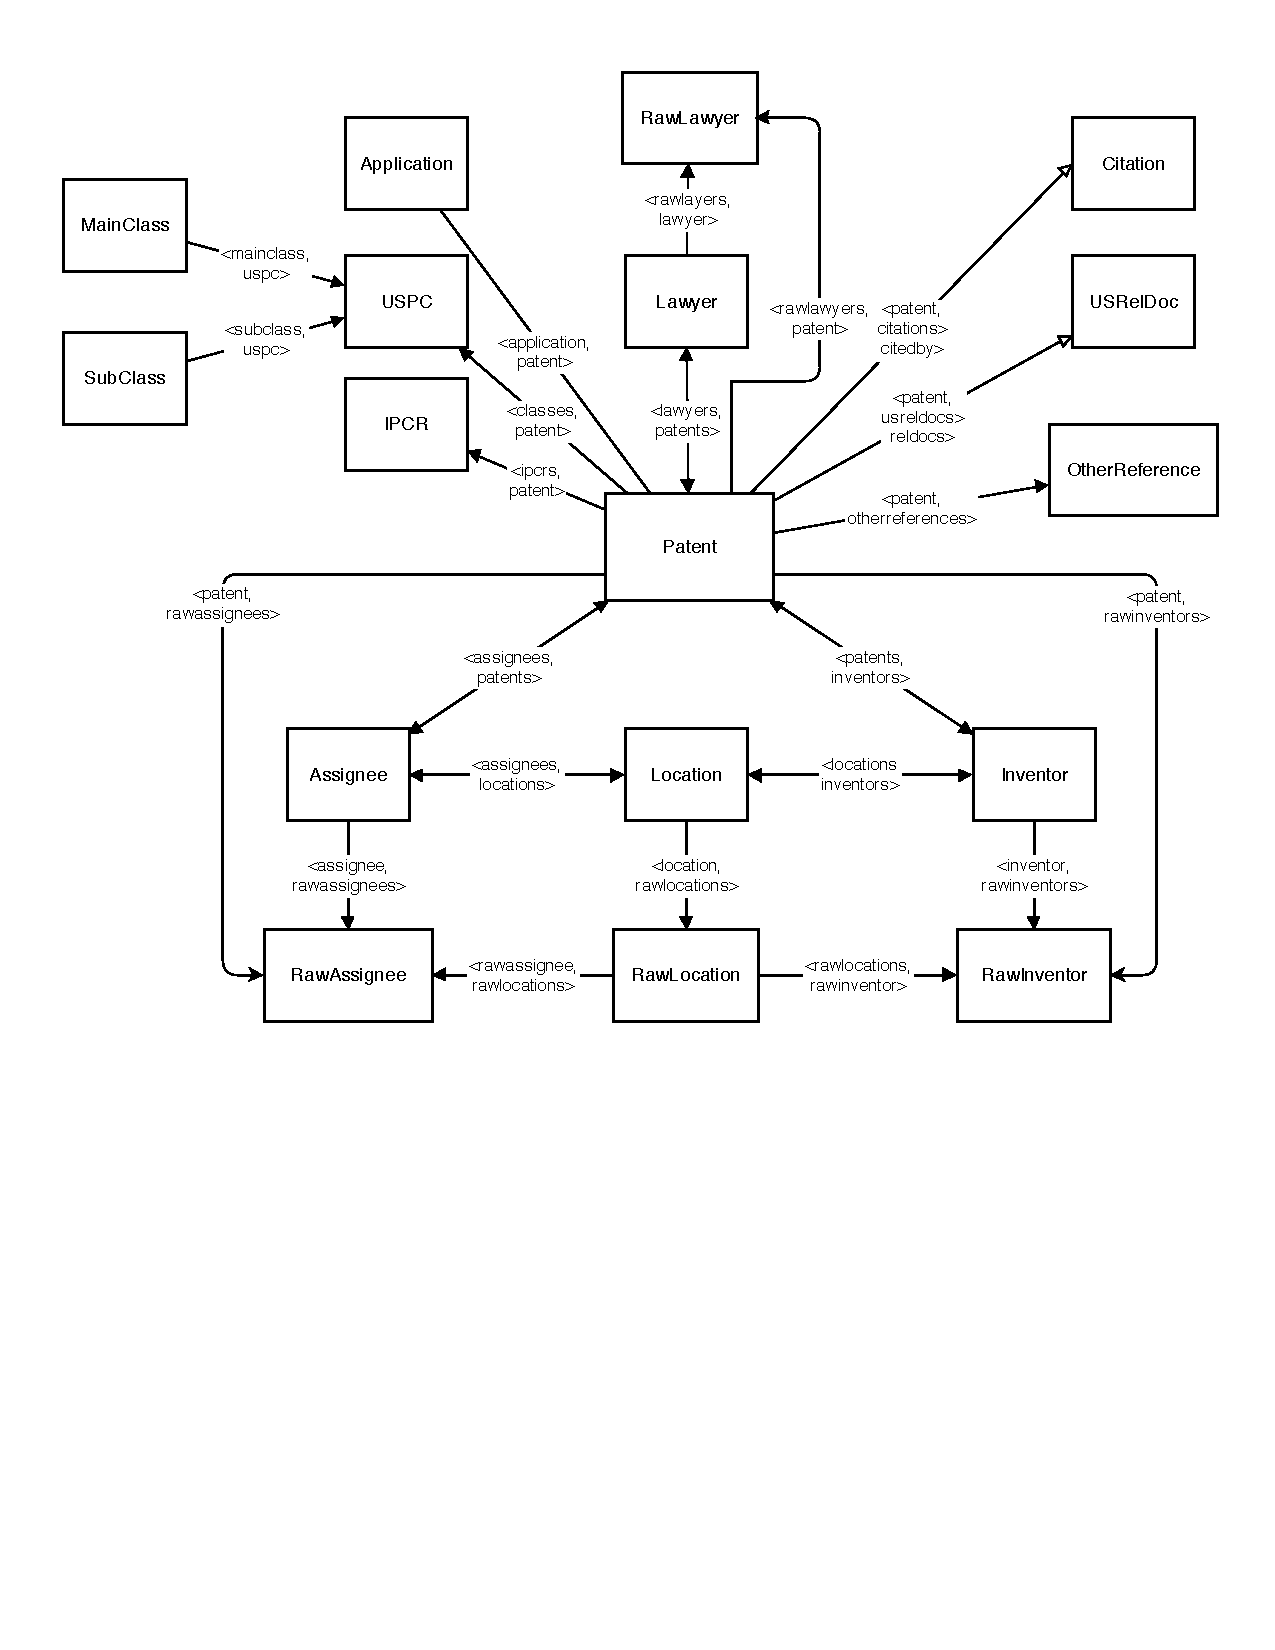
\includegraphics[width=0.6\textwidth]{figs/database-simplified}
\caption{High level view of new database schema}


\label{fig:newschema} 
\end{figure*}


We wanted to have a highly-linked database that would make it easy
for developers to access related information for a given set of patents.
The DVN schema, as described in the Appendix, does not take advantage
of foreign key relations, and places much manual burden on the user.
This was a primary motivating factor in our design, which is summarized
in Figure~\ref{fig:newschema}.


\subsection{Raw vs Processed}

If we examine the new database schema, for each of the \verb`inventor`,
\verb`lawyer`, \verb`location`, and \verb`assignee` tables, we
can see a ``raw'' version (e.g. \verb`rawinventor`) and a plain
version. The \verb`raw` tables contain the inventor, lawyer, location
and assignee records \emph{as they appear in the USPTO files}, which
means that the naming inconsistencies and misspellings are preserved.
These records are run through disambiguation methods of various degrees
of rigor, and the cleaned records are stored in the plain tables.
See below for a description of these disambiguation methods.

When the cleaned records are inserted, we link them to both the related
patent and the raw version using foreign keys in the database, so
it is simple to examine groups of related records. See Table~\ref{table:rawclean}.

\begin{table*}
\center %
\begin{tabular}{|l|l|l|}
\hline 
Table  & Access  & Value \tabularnewline
\hline 
Patent  & \verb`patent`  & US8434162 \tabularnewline
Inventor  & \verb`patent.inventors[0]`  & Thomas H. Stachler \tabularnewline
Raw Location  & \verb`patent.inventors[0].rawlocation`  & Deyton, OH, US \tabularnewline
Clean Location  & \verb`patent.inventors[0].location`  & Dayton, OH, US \tabularnewline
\hline 
\end{tabular}\caption{Accessing related raw and clean records. Note the spelling correction
in the clean record}


\label{table:rawclean} 
\end{table*}


\section{Disambiguations}
One of the primary problems with conducting meaningful research with USPTO
patent data is the high variability in quality. Cities are misspelled or
mislisted. Organizations are alternatively abbreviated and listed in full with
little modicum of consistency. Inventors, lawyers and assignees will misspell
their names, change their names and unpredictably list their middle initials or
names. The Berkeley patent database provides facilities to account for these
errors, and codifies the disambiguation of such records in order to make
possible their accurate retrieval.

\subsection{Geocoding}

There are over 12 million locations listed in the USPTO patent weekly downloads
from 1975 to 2013, with 350,000 unique tuples of \verb`(city, state, country)`.
These tuples follow the typical motif of data problems in the rest of the
patent data: incorrect or nonstandard country codes, inconsistent romanization
of foreign locations and various misspellings. We resolved the ambiguities in
the location data using a propietary disambiguation technique developed by
Google. When new patent data is processed, we run a series of data cleaning
processes to correct for some of the common errors, then cross reference with the
lookup table~\cite{geotable} obtained through the Google disambiguation.

A detailed analysis of the problems with USPTO location data and our handling
of locations can be found through a related Fung Institute
publication~\cite{geocoding}. 

Locations are associated with assignees, inventors and lawyers. Typically, a
patent record's ``location'' is the location of the first inventor listed on
the patent.

\subsection{Assignees}

For a given patent, the assignees are the entities (either organizations or
individuals) that have property rights to the patent. The assignee records are
imperative for firm-level analysis of patent data, and are used for tracking
ownership of patents. The weekly releases of patent documents only contain the
original assignee of a patent when it was initially granted.

However, it is difficult to obtain accurate results for simple (and necessary)
questions such as \emph{``which patents are owned by firm X?''} because of the
pandemic inconsistency of spellings. A cursory search for assignee records that
resemble General Electric yield the following:

\begin{itemize}
    \item General Electric Company
    \item General Electric
    \item General Electric Co..
    \item General Electric Capital Corporation
    \item General Electric Captical Corporation
    \item General Electric Canada
    \item General Electrical Company
    \item General Electro Mechanical Corp
    \item General Electronic Company
    \item General Eletric Company
\end{itemize}

This is not even a complete list of all the (mis)representations of General
Electric, but already we can see the potential issues with trying to get
accurate results.

We do not yet provide fully featured entity resolution for assignee records,
but we do maintain a preliminary disambiguation of the records that corrects
for minor misspellings. We do this by applying the Jaro-Winkler~\cite{jw}
string similarity algorithm to each pair of raw assignee records. Two records
that are within a certain bound of similarity are considered the same, and are
linked together.

It is not tractable to perform pairwise computation on each of the 5,850,531
raw assignee records in the database (at time of writing), so we group the
assignees by their first letter, and then perform the pairwise comparisions
within each of these blocks. This allows us to hold a smaller chunk of the
assignees in memory at each step, and achieves near the same accuracy.

\subsection{Lawyers}

The raw lawyer records follow much of the same deficiencies in quality as the
assignee records. Again, we only offer a preliminary disambiguation of lawyer
records using the same algorithm as described above, but future development
will yield more accurate results.

\subsection{Inventors}

We provide a polished disambiguation mechanism for inventor records. Using the
published name of an inventor, the patent technology class, co-inventor names,
published location and original assignee, we are able to infer with more than
95\% accuracy which inventor records are the same across all records in the
patent database.

A detailed summary of our technique can be found through a related Fung
Institute publication~\cite{newdisambiguation}.

\section{Statistics}
Many research applications of patent data require records from multiple
tables to be linked together: for instance, finding all citations
made to a patent, or finding all patents for an inventor. Due to the
size of the database, however, gathering all the requisite data and
linking it together takes a nontrivial amount of time. To facilitate
some common research vectors, we provide three tables of precompiled
statistics.

The \verb`FutureCitationRank` table contains the rank of each patent
by the number of future citations in each year. This answers the question
``in year X, patent number Y got Z citations. It was the Nth most
cited patent that year''.

The \verb`InventorRank` table contains the rank of each inventor
by how many patents they have been granted in a given year.

The \verb`CitedBy` table contains the direct mapping of a focal patent
to all patents that cite that patent. 


{
\scriptsize
\bibliographystyle{acm}
\bibliography{patentprocessor}
}

%\clearpage
\section*{Appendix}
\subsection*{Harvard DVN Database Schemas}

\begin{table}[ht]
\center
\begin{tabular}{| l | l |}
\hline
Column Name & Column Description \\
\hline
\verb`Patent` & Patent owned by assignee \\
\verb`AsgType` & Unknown \\
\verb`Assignee` & Name of assignee \\
\verb`City` & City location of assignee \\
\verb`State` & State location of assignee \\
\verb`Country` & Country of assignee \\
\verb`Nationality` & Nationality of assignee \\
\verb`Residence` & Street address of assignee \\
\verb`AsgSeq` & Order of assignee as appears in patent \\
\hline
\end{tabular}
\caption{DVN table schema for assignees}
\end{table}

\begin{table}[ht]
\center
\begin{tabular}{| l | l |}
\hline
Column Name & Column Description \\
\hline
\verb`Patent` & Patent making the citation \\
\verb`Cit_Date` & Date of cited document \\
\verb`Cit_Name` & Unknown \\
\verb`Cit_Kind` & Type of cited document \\
\verb`Cit_Country` & Origin of cited document \\
\verb`Citation` & Number or ID of cited document \\
\verb`Category` & Unknown \\
\verb`CitSeq` & Order of citation as appears in patent \\
\hline
\end{tabular}
\caption{DVN table schema for citations}
\end{table}

\begin{table}[ht]
\center
\begin{tabular}{| l | l |}
\hline
Column Name & Column Description \\
\hline
\verb`Patent` & focal Patent \\
\verb`Prim` & Order of classification \\
\verb`Class` & USPTO technology class \\
\verb`SubClass` & USPTO technology subclass \\
\hline
\end{tabular}
\caption{DVN table schema for classes}
\end{table}

\begin{table}[ht]
\center
\begin{tabular}{| l | l |}
\hline
Column Name & Column Description \\
\hline
\verb`Patent` & Patent owned by inventor \\
\verb`Firstname` & Inventor's first name \\
\verb`Lastname` & Inventor's last name \\
\verb`Street` & Inventor street address \\
\verb`City` & Inventor city \\
\verb`State` & Inventor state \\
\verb`Country` & Inventor country \\
\verb`Zipcode` & Inventor zipcode \\
\verb`Nationality` & Inventor nationality \\
\verb`InvSeq` & Order of inventor as listed on patent \\
\hline
\end{tabular}
\caption{DVN table schema for inventors}
\end{table}

\begin{table}[ht]
\center
\begin{tabular}{| l | l |}
\hline
Column Name & Column Description \\
\hline
\verb`Patent` & Patent number \\
\verb`Kind` & Unknown \\
\verb`Claims` & Number of claims made by patent \\
\verb`AppType` & Unknown \\
\verb`AppNum` & Application reference number \\
\verb`GDate` & Date of grant \\
\verb`GYear` & Year of grant \\
\verb`AppDate` & Date of application \\
\verb`AppYear` & Year of application \\
\verb`PatType` & Type of patent (Reissue, Utility, etc) \\
\hline
\end{tabular}
\caption{DVN table schema for patents}
\end{table}

\begin{table}[ht]
\center
\begin{tabular}{| l | l |}
\hline
Column Name & Column Description \\
\hline
\verb`Patent` & focal Patent \\
\verb`Abstract` & Patent abstract \\
\verb`Title` & Patent title \\
\hline
\end{tabular}
\caption{DVN table schema for patent descriptions}
\end{table}

\begin{table}[ht]
\center
\begin{tabular}{| l | l |}
\hline
Column Name & Column Description \\
\hline
\verb`Patent` & focal Patent \\
\verb`Firstname` & Lawyer's first name \\
\verb`Lastname` & Lawyer's last name \\
\verb`LawCountry` & Location of lawyer \\
\verb`OrgName` & Name of law firm or organization \\
\verb`LawSeq` & Order of lawyer as listed in patent \\
\hline
\end{tabular}
\caption{DVN table schema for lawyers}
\end{table}

\begin{table}[ht]
\center
\begin{tabular}{| l | l |}
\hline
Column Name & Column Description \\
\hline
\verb`Patent` & focal Patent \\
\verb`Descrip` & Description of scientific reference \\
\verb`CitSeq` & Order of citation as appears in patent \\
\hline
\end{tabular}
\caption{DVN table schema for scientific references}
\end{table}

\begin{table}[ht]
\center
\begin{tabular}{| l | l |}
\hline
Column Name & Column Description \\
\hline
\verb`Patent` & focal Patent \\
\verb`DocType` & Type of related document \\
\verb`OrderSeq` & Order of document as appears in patent \\
\verb`Country` & Country of origin for related document \\
\verb`RelPatent` & Patent number of related document \\
\verb`Kind` & Unknown \\
\verb`RelDate` & Date of related document \\
\verb`Status` & Status of related document \\
\hline
\end{tabular}
\caption{DVN table schema for US related documents}
\end{table}


\end{document}
